\documentclass[12pt]{article}
\usepackage{amsmath}
\usepackage{latexsym}
\usepackage{amsfonts}
\usepackage[normalem]{ulem}
\usepackage{soul}
\usepackage{array}
\usepackage{amssymb}
\usepackage{extarrows}
\usepackage{graphicx}
\usepackage[backend=biber,
style=numeric,
sorting=none,
isbn=false,
doi=false,
url=false,
]{biblatex}\addbibresource{bibliography-biblatex.bib}

\usepackage{subfig}
\usepackage{wrapfig}
\usepackage{txfonts}
\usepackage{wasysym}
\usepackage{enumitem}
\usepackage{adjustbox}
\usepackage{ragged2e}
\usepackage[svgnames,table]{xcolor}
\usepackage{tikz}
\usepackage{longtable}
\usepackage{changepage}
\usepackage{setspace}
\usepackage{hhline}
\usepackage{multicol}
\usepackage{tabto}
\usepackage{float}
\usepackage{multirow}
\usepackage{makecell}
\usepackage{fancyhdr}
\usepackage[toc,page]{appendix}
\usepackage[hidelinks]{hyperref}
\usetikzlibrary{shapes.symbols,shapes.geometric,shadows,arrows.meta}
\tikzset{>={Latex[width=1.5mm,length=2mm]}}
\usepackage{flowchart}\usepackage[paperheight=11.69in,paperwidth=8.27in,left=1.18in,right=0.79in,top=1.68in,bottom=1.37in,headheight=1in]{geometry}
\usepackage[utf8]{inputenc}
\usepackage[T1]{fontenc}
\TabPositions{0.5in,1.0in,1.5in,2.0in,2.5in,3.0in,3.5in,4.0in,4.5in,5.0in,5.5in,6.0in,}
\urlstyle{same}


 %%%%%%%%%%%%  Set Depths for Sections  %%%%%%%%%%%%%%

% 1) Section
% 1.1) SubSection
% 1.1.1) SubSubSection
% 1.1.1.1) Paragraph
% 1.1.1.1.1) Subparagraph


\setcounter{tocdepth}{5}
\setcounter{secnumdepth}{5}


 %%%%%%%%%%%%  Set Depths for Nested Lists created by \begin{enumerate}  %%%%%%%%%%%%%%


\setlistdepth{9}
\renewlist{enumerate}{enumerate}{9}
		\setlist[enumerate,1]{label=\arabic*)}
		\setlist[enumerate,2]{label=\alph*)}
		\setlist[enumerate,3]{label=(\roman*)}
		\setlist[enumerate,4]{label=(\arabic*)}
		\setlist[enumerate,5]{label=(\Alph*)}
		\setlist[enumerate,6]{label=(\Roman*)}
		\setlist[enumerate,7]{label=\arabic*}
		\setlist[enumerate,8]{label=\alph*}
		\setlist[enumerate,9]{label=\roman*}

\renewlist{itemize}{itemize}{9}
		\setlist[itemize]{label=$\cdot$}
		\setlist[itemize,1]{label=\textbullet}
		\setlist[itemize,2]{label=$\circ$}
		\setlist[itemize,3]{label=$\ast$}
		\setlist[itemize,4]{label=$\dagger$}
		\setlist[itemize,5]{label=$\triangleright$}
		\setlist[itemize,6]{label=$\bigstar$}
		\setlist[itemize,7]{label=$\blacklozenge$}
		\setlist[itemize,8]{label=$\prime$}



 %%%%%%%%%%%%  Header here  %%%%%%%%%%%%%%


\pagestyle{fancy}
\fancyhf{}
\lhead{ \setlength{\parskip}{0.0pt}

\vspace{\baselineskip}
\setlength{\parskip}{12pt}
}
\lfoot{ 
\vspace{\baselineskip}
\setlength{\parskip}{0.0pt}
\setlength{\parskip}{12pt}

\vspace{\baselineskip}
\setlength{\parskip}{0.0pt}
\setlength{\parskip}{12pt}
}
\renewcommand{\headrulewidth}{0pt}
\setlength{\topsep}{0pt}\setlength{\parskip}{9.96pt}
\setlength{\parindent}{0pt}


 %%%%%%%%%%%%  Footer Here  %%%%%%%%%%%%%%

\usepackage{fancyhdr}
\pagestyle{fancy}
\fancyhf{}
\fancyfoot[CE,CO]{Department of Electronics and Telecommunication}
\fancyfoot[LE,RO]{\thepage}

 %%%%%%%%%%%%  This sets linespacing (verticle gap between Lines) Default=1 %%%%%%%%%%%%%%


\renewcommand{\arraystretch}{1.3}


%%%%%%%%%%%%%%%%%%%% Document code starts here %%%%%%%%%%%%%%%%%%%%



\begin{document}
\begin{Center}
{\fontsize{18pt}{21.6pt}\selectfont \textbf{Chapter 1 - Introduction}}
\end{Center}
\vspace{\baselineskip}
\vspace{\baselineskip}

\setstretch{1}
\begin{justify}
{\fontsize{14pt}{16.8pt}\selectfont \textbf{1.1 Introduction and need of the project}}
\vspace{\baselineskip}

\end{justify}
\setlength{\parskip}{0.0pt}
\begin{justify}
Humans tend to neglect basic safety measures like practicing social distancing and wearing a mask to ensure safety of others. We tend to neglect basic hygiene like use of sanitizers, practicing human contact like handshakes without ensuring sanitary condition. Countless diseases are caused by microorganisms that persist by infecting new people. Cutting these detrimental interactions in public would enable us to eliminate ailments before they grow to be a pandemic. Such measures are essential considering the fact that even extremely common diseases like the common cold can make a perfectly healthy person ill purely based on an asymptomatic interaction that lasted a few seconds.
\end{justify}

\vspace{\baselineskip}
\setlength{\parskip}{9.96pt}
\setlength{\parskip}{0.0pt}
\begin{justify}
The proposed system has two independent parts referred to as the active and the passive part. The system has been designed in such a way to compensate for the fact that not every interaction calls for action. Only certain interactions and unhealthy practices need to be flagged to the authorities and the user itself.The\ main stages of the Disease  Assistant are, data acquisition, synthesis and implementation. Hence, a CCTV camera network is used to record the human traffic in public places and detect the patterns and the proximity of one subject with another. Other than this, there are algorithms which account for the environmental conditions like temperature and humidity. Along with this, wearing a mask will account for the final $``$risk factor$"$  for each individual in consideration .It\ Consists\ of\ a  camera and multiple deep learning algorithms that calculate risk factor. If the risk factor is  high for any particular person, the active module comes into effect and suggests solutions and  precautions along with an option to book doctor appointments.
\end{justify}

\vspace{\baselineskip}
\setlength{\parskip}{9.96pt}
\setlength{\parskip}{0.0pt}
\begin{justify}
 \tab In case the risk factor, an individual will have to submit their reports and other medical details to a flask chatbot before visiting the doctor.The interactive flask based chatbot provides an easy and effective user interface. If a medical consultation is deemed essential by the algorithms, only then will the person need to consult a doctor. For this, he will be given a list of authorised doctors in his locality and the timings on which they will be available for consultation. Booking an appointment and the update to the doctor along with all the reports will be sent automatically to ensure there is no added pressure on the medical fields and the system relieves pressure that medical practitioners face during a surge in patient numbers.
\end{justify}

\vspace{\baselineskip}
\setlength{\parskip}{9.96pt}
\setlength{\parskip}{0.0pt}
\vspace{\baselineskip}
\vspace{\baselineskip}
\vspace{\baselineskip}
\vspace{\baselineskip}
\vspace{\baselineskip}
\vspace{\baselineskip}

{\fontsize{14pt}{16.8pt}\selectfont \textbf{1.2 Problem statement in broad sense }}
\vspace{\baselineskip}
\vspace{\baselineskip}
\begin{justify}
A disease becomes a pandemic upon negligence and high infectivity.Thereby finding an effective and efficient solution is critical so as to avoid escalation of a communicable ailment that may gradually lead to a pandemic scenario. This system can be successfully implemented as safety and an effective preventive system.{\fontsize{14pt}{16.8pt}\selectfont \textbf{ }}With this project we aim at developing a self sustaining system which helps relieve the pressure faced by medical practitioners in the long run, while ensuring that hygiene is maintained in public places.
\end{justify}

\vspace{\baselineskip}
\setlength{\parskip}{9.96pt}
\setlength{\parskip}{0.0pt}
\begin{justify}
 In some Asian countries like Japan, it is mandated to follow the rules we’re trying to enforce when a person suffers from any communicable ailments. We saw the Covid-19 virus become a worldwide pandemic, many researches suggest that COVID could be a start to many harder to deal viruses to come. Hence it is essential that in the future, these diseases are healed before gain enough infectivity to become a pandemic.The project identifies variable factors influencing public hygiene and discrepancies in the healthcare system.The system can be further modified to successfully target a specific disease very easily and ensure maximum accuracy and quick adaptation.
\end{justify}

\vspace{\baselineskip}
\setlength{\parskip}{9.96pt}

\vspace{\baselineskip}
\setlength{\parskip}{0.0pt}
\setlength{\parskip}{9.96pt}

\vspace{\baselineskip}
\setlength{\parskip}{0.0pt}
\setlength{\parskip}{9.96pt}

\vspace{\baselineskip}
\setlength{\parskip}{0.0pt}
\setlength{\parskip}{9.96pt}

\vspace{\baselineskip}
\setlength{\parskip}{0.0pt}
\setlength{\parskip}{9.96pt}

\vspace{\baselineskip}
\setlength{\parskip}{0.0pt}
\setlength{\parskip}{9.96pt}

\vspace{\baselineskip}
\setlength{\parskip}{0.0pt}
\setlength{\parskip}{9.96pt}

\vspace{\baselineskip}
\setlength{\parskip}{0.0pt}
\setlength{\parskip}{9.96pt}

\vspace{\baselineskip}
\setlength{\parskip}{0.0pt}
\setlength{\parskip}{9.96pt}

\vspace{\baselineskip}
\setlength{\parskip}{0.0pt}
\setlength{\parskip}{9.96pt}

\vspace{\baselineskip}
\setlength{\parskip}{0.0pt}
\setlength{\parskip}{9.96pt}

\vspace{\baselineskip}
\setlength{\parskip}{0.0pt}
\setlength{\parskip}{9.96pt}
\setlength{\parskip}{0.0pt}
\vspace{\baselineskip}
\vspace{\baselineskip}
\vspace{\baselineskip}
\vspace{\baselineskip}
\vspace{\baselineskip}
\vspace{\baselineskip}
\vspace{\baselineskip}
\vspace{\baselineskip}
\vspace{\baselineskip}
\vspace{\baselineskip}
\vspace{\baselineskip}
\vspace{\baselineskip}
\vspace{\baselineskip}
\vspace{\baselineskip}
\vspace{\baselineskip}

\begin{justify}
{\fontsize{14pt}{16.8pt}\selectfont \textbf{1.3 Organization of the report}}
\end{justify}

\vspace{\baselineskip}
\setlength{\parskip}{9.96pt}
\begin{FlushLeft}
The report is divided into five chapters. Each part deals with the different stages of the \textbf{Disease Assistant }. Each chapter has various parts explaining in detail
\end{FlushLeft}
\begin{FlushLeft}
\textbf{\\
\tab Chapter 2} provides a foundation of knowledge on the topic, identifies areas of prior scholarship to prevent duplication and give credit to other researchers. It also identifies inconsistencies: gaps in research, conflicts in previous studies, open questions left from other research. It also discusses the need for additional research to justify our research and identifies the relationship of works in context of its contribution to the topic and to other works. It places our current research within the context of existing literature making a case for why further study is needed.
\end{FlushLeft}
\setlength{\parskip}{12.0pt}
\textbf{Chapter 3 }discusses the team’s work on the project and step by step development. It discusses the objectives in mind while developing the system. It also discusses the system hardware architecture and software design.\textbf{ }Next, it describes the methodology in detail of each working part of the system. And finally it describes the implementation techniques and deployment scenarios.
\textbf{Chapter 4 }discusses the results and output, and how they are to be deployed in the real world.\textbf{ }It starts by talking about the passive model which is abstracted at deployment. Finally, it talks about the active model UI, implementation and UX.

\vspace{\baselineskip}
\setlength{\parskip}{9.96pt}
\begin{FlushLeft}
Finally, \textbf{Chapter 5} concludes the thesis and discusses some future work.
\end{FlushLeft}

\vspace{\baselineskip}
\setstretch{2.0}

\vspace{\baselineskip}

\vspace{\baselineskip}

\vspace{\baselineskip}

\vspace{\baselineskip}
\vspace{\baselineskip}
\vspace{\baselineskip}
\vspace{\baselineskip}
\vspace{\baselineskip}
\vspace{\baselineskip}
\vspace{\baselineskip}

\begin{Center}
{\fontsize{18pt}{21.6pt}\selectfont \textbf{Chapter 2 - Literature review}}
\end{Center}
\setstretch{1}
\setlength{\parskip}{12.0pt}
\begin{justify}
 \tab In recent years, the architectures based on the convolution neural network (CNN) results showed major improvements in performance which contribute to the high quality of object detection. A feasible method that consists of first identifying facial features has been proposed. The issue of occluded face detection was solved using the Multi-Task Cascaded Convolutional Neural Network (MTCNN). Extraction of facial features is then carried out using the embedding model of Google FaceNet embedded model. Eventually, the Support Vector Machine (SVM) has conducted the classification task.[1] Because the model offers better accuracy for simple masked face recognition and can not be appeased for all forms of masks, the proposed project has a trained custom dataset model that includes complex and many more occlusion sources, including hat, sunglasses, beard, long hair, mustache, and medicine. In static images, as well as in real time video streams, it can detect face masks. 
\end{justify}
\begin{justify}
 \tab A\ study[2] was suggested that uses object detection and tracking models to help deal with the worsening of COVID-19 cases in the social distancing remedy. The research uses the YOLO v3 object detection model to isolate humans from the background and to monitor the detected individuals using bounding boxes and assigned IDs using the Deepsort method. The pairwise vectorized L2 standard is later determined on the basis of the three-dimensional space of the function obtained by using the centroid coordinates and the bounding box dimensions. To measure the non-adoption of the social distancing protocol, the breach index  or violation index term is suggested.
\end{justify}
\begin{justify}
 A similar project suggested a deep learning solution that would warn the user as soon as social distance is breached. A video stream is taken from the CCTV camera and the individuals are detected with the PoseNet model and then a rack is maintained of the number of people in the video stream. If the difference between 2 people's frames is less then the authorities in charge are alerted[3]. Since both approaches are highly sensitive to the spatial location of the camera and intended to be used in any working environment; accuracy and precision are highly desired to serve the purpose and to avoid discomfort and panic situations among people. The proposed project detects the social distancing and masks with a precision and confidence score that reduces the number of false positives. The passive model operates two tasks: firstly, face mask detection secondly; the detection of a social distance violation by individuals is detected continuously in threshold time by using a sliding window on a fast R-CNN to get maximum efficiency output. This solution can be used in places like temples, shopping complexes, metro stations, airports, etc.
\end{justify}
\begin{justify}
Community participation is the first line of protection in the conflict against infectious diseases and an important role is provided by general practitioners (GPs). The study analyzed the key problems that need to be addressed, planned and developed a dynamic risk assessment decision support framework for COVID-19 (DDC19) [4] centered on the real scenes and processes of patients using health care. The developed DDC19 consists of three components: two main mobile terminal applications (patient end $\&$  GP end), a database system with related components and a related support model underlying it. All mobile terminal devices are wirelessly linked to the back-end data center to send requests and transmit data. A multi-class logistic regression algorithm, a 10-fold cross-validation approach to evaluate and test the COVID-19 dynamic risk stratification model in various scenarios, is allocated as labels for the three groups of low risk, moderate risk and high risk.The system is still in the deployment and app stage, the relevant data of patients in the system and in-hospital visits cannot be obtained in a timely manner including the severity of symptoms and history of underlying chronic diseases and majorly does not include any real time communication to seek constant advice. While our projects aim at Python - Flask chat bot to collect essential data and seek emergency appointments at the hospital. When the risk calculation gives very high risk for a particular person, he is sent a link via mail to an AI Chatbot. The real time parameter that is symptom checker considers various parameters including temperature Screening which is another key symptom of COVID-19 infection.
\end{justify}

\vspace{\baselineskip}
\setlength{\parskip}{9.96pt}

\vspace{\baselineskip}

\vspace{\baselineskip}

\vspace{\baselineskip}

\vspace{\baselineskip}

\vspace{\baselineskip}
\setstretch{2.0}

\vspace{\baselineskip}
\vspace{\baselineskip}
\vspace{\baselineskip}
\vspace{\baselineskip}
\vspace{\baselineskip}
\vspace{\baselineskip}
\vspace{\baselineskip}
\vspace{\baselineskip}
\vspace{\baselineskip}
\vspace{\baselineskip}
\vspace{\baselineskip}
\vspace{\baselineskip}

\begin{Center}
{\fontsize{18pt}{21.6pt}\selectfont \textbf{Chapter 3 - Report on Present Investigation}}
\vspace{\baselineskip}

\end{Center}
\begin{FlushLeft}
{\fontsize{14pt}{16.8pt}\selectfont \textbf{3.1 Objectives }}
\end{FlushLeft}
\setstretch{1}
\begin{FlushLeft}
With this project we aim at developing a self sustaining system which helps relieve the pressure faced by medical practitioners in the long run. The project identifies variable factors influencing public hygiene and discrepancies in the healthcare system. The system can be further modified to successfully target a specific disease very easily and ensure maximum accuracy and quick adaptation. A disease becomes a pandemic upon negligence and high infectivity. This system can be successfully implemented as safety and an effective preventive system.
\end{FlushLeft}

\vspace{\baselineskip}
\setstretch{2.0}
\begin{justify}
{\fontsize{14pt}{16.8pt}\selectfont \textbf{3.2 System Architecture and Design}}
\end{justify}
\vspace{\baselineskip}
\setstretch{1}
\setlength{\parskip}{0.0pt}
\begin{justify}
A CCTV camera network / webcam (Pixel resolution is 1280 x 1024 (like the Sony SNC-EM600 1.3 megapixel camera), or it can be 1280 x 800, 1080p cameras that have at least a 2-megapixel sensor, to capture the video of the people moving in a office or open environment.
\end{justify}

\vspace{\baselineskip}
\setlength{\parskip}{9.96pt}
\setlength{\parskip}{0.0pt}
\begin{justify}
In\ their paper, "Rapid Object Detection using a Boosted Cascade of Simple Features" in 2001, Object Detection using Haar feature-based cascade classifiers is an efficient object detection method proposed by Paul Viola and Michael Jones. To obtain the bounding box coordinates of faces in an image, we will be using a Haar Cascade Model trained to detect faces. Face Mask Detection system built with OpenCV, Keras/TensorFlow. We use the MobilenetV2 in transfer learning. We remove the bottom few layers worth of weights from the pre-existing model and add a flatten and a dense layer with 2 output neurons specifying $``$with and without$"$  masks. Next for social distancing checking, which can be done by iterating over the coordinates of faces and calculating the distance for each possible pair, if the distance for a particular pair is less than  the threshold then the bounding boxes for those faces are colored red. Threshold must be manually initialized in such a way that it corresponds to the minimum allowable distance in real life (ex. 6ft in India). In addition to this, we’ll use a sliding window on a fast R-CNN to get maximum efficiency output. The CNN will extract the features and the classifier - regressor stack will calculate the distance at maximum accuracy. State-of-the-art object detection networks to hypothesise object coordinates rely on area proposal algorithms. The running time of these detection networks has been reduced by developments such as SPPnet and Fast R-CNN, identifying region proposal computation as a bottleneck.
\end{justify}

\vspace{\baselineskip}
\setlength{\parskip}{9.96pt}
\setlength{\parskip}{0.0pt}
\begin{justify}
Also Detectron 2.0 was used and combined with the Haar cascade model, the Haar cascade model works effectively but gives error as it takes into account only persons standing in a straight line to overcome this, we combine it with Detectron 2.0 which gives us the birds eye view of the frame and calculates the distance between two persons effectively. The Detectron 2.0 is a collective object detection model which is an open source model built by FAIR that is the Facebook AI and Research and helps in object detection. It is implemented from the Detectron Model Zoo which has various pretrained models, transfer learning is applied on one particular model to obtain the desired results. An interactive chatbot will be built using Python-Flask. The reason we chose flask as the web development framework is that our complete system is coded in python. So any and all code will directly work on the framework without any major modifications.
\end{justify}

\vspace{\baselineskip}
\setlength{\parskip}{9.96pt}
\setlength{\parskip}{0.0pt}
\begin{justify}
The\ Telegram BotFather API is used to build a chatbot as it has built in features to interact with the user. When the risk calculation gives very high risk for a particular person, he is sent a link on the contact information provided to an AI Chatbot. Collecting information from the user, the chatbot will suggest best possible measures going forward and help in booking a doctor appointment if need be. There is a frontend booking page developed using flask  which shows all available doctors in a particular location and the slots when they’re free to be able to book an appointment without any hassle. Also the doctors can create new slots in the appointment booking portal according to their schedule.
\end{justify}

\vspace{\baselineskip}
\setlength{\parskip}{9.96pt}

\vspace{\baselineskip}
\setstretch{2.0}

\vspace{\baselineskip}

\vspace{\baselineskip}
\vspace{\baselineskip}
\vspace{\baselineskip}
\vspace{\baselineskip}
\vspace{\baselineskip}
\vspace{\baselineskip}
\vspace{\baselineskip}
\vspace{\baselineskip}
\vspace{\baselineskip}
\vspace{\baselineskip}
\vspace{\baselineskip}
\vspace{\baselineskip}

\begin{FlushLeft}
{\fontsize{14pt}{16.8pt}\selectfont \textbf{3.3 Algorithm:}}
\end{FlushLeft}
\begin{FlushLeft}
{\fontsize{13pt}{15.6pt}\selectfont \textbf{3.3.1 Passive model algorithm:}}
\end{FlushLeft}
\setstretch{1}
\begin{justify}
Input\ is\ taken\ from\ the\ camera\ and\ is\ used for detecting facial masks and to calculate a risk factor. The video is split into workable frames and bounding boxes are obtained  using HAAR cascade. Transfer learning is  applied on Mobilenet V2 to detect the presence of  a facial mask. Results are obtained and objects are classified as wearing masks and not wearing masks. The Input video is split in frames and Detectron 2.0 is applied over each frame. To increase the accuracy we use a birds eye view  model. The Birds eye model is used to  obtain accurate object detection by generating a top view perspective of an image. The midpoint of bounding boxes is calculated with  each point representing  a particular person. Proximity is calculated using euclidean distance for each possible point pair. If the proximity values are below a certain threshold then they are considered as unhealthy interaction and marked as red. If the risk factor comes out to be high  then the active model starts working.
\end{justify}

\vspace{\baselineskip}
\begin{FlushLeft}
{\fontsize{14pt}{16.8pt}\selectfont \textbf{3.3.2 Active model algorithm:}}
\end{FlushLeft}
\begin{justify}
A\ link to an interactive Telegram chatbot is sent to the person having a high risk factor via mail. The user is provided with  a unique CDA-ID\ using\ which\ the\ chatbot identifies the person. Basic information is collected by the chatbot regarding the patient health conditions. It recognises the patients  conditions and starts  providing  suggestions accordingly. It even provides an option to book an appointment with  a doctor. In case the user wants to book an appointment, he is asked to register using a userID and password.The available slots are displayed in green and booked ones are indicated in red.After booking a slot the booked slots are successfully reflected on the slot booking page.
\end{justify}

\vspace{\baselineskip}
\setstretch{2.0}

\vspace{\baselineskip}

\vspace{\baselineskip}
\vspace{\baselineskip}
\vspace{\baselineskip}
\vspace{\baselineskip}
\vspace{\baselineskip}
\vspace{\baselineskip}

\begin{FlushLeft}
{\fontsize{14pt}{16.8pt}\selectfont \textbf{3.4 Methodology}}
\end{FlushLeft}
\begin{FlushLeft}
The overall framework of the proposed model is shown below:
\end{FlushLeft}


%%%%%%%%%%%%%%%%%%%% Figure/Image No: 2 starts here %%%%%%%%%%%%%%%%%%%%

\begin{figure}[H]
	\begin{Center}
		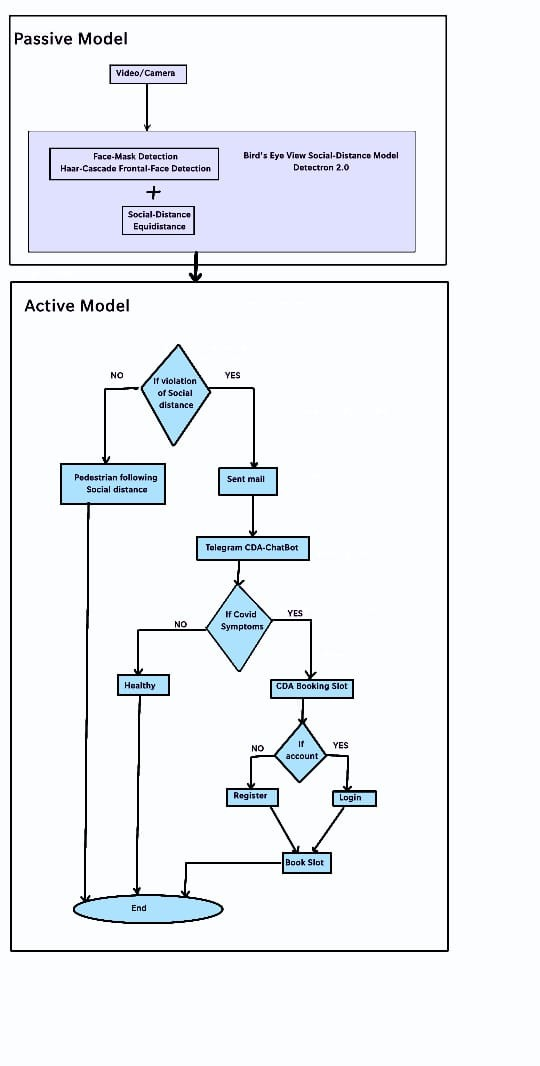
\includegraphics[width=4.32in,height=7in]{./media/image4.png}
	\end{Center}
\end{figure}


%%%%%%%%%%%%%%%%%%%% Figure/Image No: 2 Ends here %%%%%%%%%%%%%%%%%%%%

\setstretch{1.0}
\setlength{\parskip}{0.0pt}

\begin{Center}
{\fontsize{14pt}{16.8pt}\selectfont Fig 1 : Project flowchart}
\end{Center}

\vspace{\baselineskip}
\setlength{\parskip}{9.96pt}
\begin{justify}
{\fontsize{14pt}{16.8pt}\selectfont \textbf{3.4.1 Passive model Methodology}}
\end{justify}
\vspace{\baselineskip}

\begin{justify}
This consists of 2 models one for facial mask recognition and one for social distancing parameters. We used Haar feature-based cascade classifiers for Object. \textcolor[HTML]{202124}{HAAR Cascade} is an object detection \textcolor[HTML]{202124}{algorithm} proposed by Paul Viola and Michael Jones to identify objects in an image or video and based on the concept of ​​ features. This is basically a machine learning based approach where a \textcolor[HTML]{202124}{cascade}\ function is trained using both positive and negative images  .Later it is used to detect the objects in the other images. To obtain the bounding box coordinates of faces in an image, we will be using a Haar Cascade Model trained to detect faces. 
\end{justify}
\begin{justify}
We use the MobilenetV2 in transfer learning.It is a multi-layered CNN.Data sets having a very large number of images can be used in it for image classification and mobile vision. \textcolor[HTML]{202124}{MobileNet}\ special uses very little computation power to run or apply transfer learning to it. We remove the bottom few layers worth of weights from the pre-existing model and add a flatten and a dense layer with 2 output neurons specifying $``$with and without'' masks. The social distancing is calculated by iterating it  over the coordinates of faces and calculating the distance for each possible pair, if the distance for a particular pair is less than the threshold then the bounding boxes for those faces are colored red. 
\end{justify}
\setlength{\parskip}{0.0pt}
\begin{justify}
Although\ the\ Haar cascade and MobileNetV2 model gave us the required facial recognition we added a birds eye model view to further increase the accuracy. Bird Eye View transformation technique is used  to generate a top view perspective of an image. This technique can be classified under digital image processing as geometrical image modification. Basically the bird’s eye view has 3 parts, first we have to represent the image in a shifted coordinate system, next perform rotation of image, and then project the image on a two dimensional plane.In the beginning the entire area is divided into  workable frames. Next we identify the number of persons in each frame. This is followed by finding proximity between individual subjects and marking them. If any person is found out violating the safe social distancing parameter a red box appears around them.
\end{justify}

\vspace{\baselineskip}
\setlength{\parskip}{9.96pt}
\begin{justify}
In addition to this we have a symptom checker which calculates a risk factor based on factors such as social and general hygiene,pre existing conditions,frequency of human interactions etc of a person .If the risk factor is above a specified safety value th then the active model starts to work and the the user is directed to a user friendly interactive chatbot.The passive models have been run and deployed on cloud. Specific changes can be done in order to improve the accessibility as well as scalability of the system if required.
\end{justify}

\vspace{\baselineskip}
\setlength{\parskip}{0.0pt}
\setlength{\parskip}{9.96pt}
\setlength{\parskip}{0.0pt}
\vspace{\baselineskip}
\vspace{\baselineskip}
\vspace{\baselineskip}
\vspace{\baselineskip}
\vspace{\baselineskip}

\begin{justify}
{\fontsize{14pt}{16.8pt}\selectfont \textbf{3.4.2 Active model Methodology}}
\end{justify}
\vspace{\baselineskip}
\begin{justify}
Any\ person having a risk factor above a certain threshold is sent a mail containing the link to an interactive chatbot. It is a Telegram Chatbot  implemented using BotFather. Users can interact with bots by sending them messages, inline\href{https://core.telegram.org/bots#inline-mode}{ }requests\ and commands. One can even control the bots using HTTPS requests to the  Bot Api.Each user has a unique CDA-ID using which the chatbot identifies the person.It asks a set of basic information gathering questions including the patient's health conditions.It recognises the conditions and starts providing suggestion. If the user replies as not feeling well then the person is directed to a flask based appointment booking slot .
\end{justify}

\vspace{\baselineskip}
\setlength{\parskip}{9.96pt}
\setlength{\parskip}{0.0pt}
\begin{justify}
The\ slot\ is created using  Python-Flask and has an attractive frontend created using HTML and CSS.At first the user need to register themselves using a userID, password.After registering the  user has an option to choose a suitable time slot which is available.The booked slots are displayed using red slots and the available slots are shown using green.The slot editing rights remain with the admin in case of cancellation of appointments,increasing or decreasing number of slots.Booking an appointment and the update to the doctor along with all the reports will be sent automatically to ensure there is no added pressure on the medical practitioners face during a surge in patient numbers. Once a particular slot has been booked the changes are successfully reflected on the slot booking page.
\end{justify}

\vspace{\baselineskip}
\setlength{\parskip}{9.96pt}

\vspace{\baselineskip}
\setlength{\parskip}{0.0pt}
\setlength{\parskip}{9.96pt}

\vspace{\baselineskip}
\setlength{\parskip}{0.0pt}
\setlength{\parskip}{9.96pt}

\vspace{\baselineskip}
\setlength{\parskip}{0.0pt}
\setlength{\parskip}{9.96pt}

\vspace{\baselineskip}
\setlength{\parskip}{0.0pt}
\setlength{\parskip}{9.96pt}

\vspace{\baselineskip}
\setlength{\parskip}{0.0pt}
\setlength{\parskip}{9.96pt}

\vspace{\baselineskip}
\setlength{\parskip}{0.0pt}
\setlength{\parskip}{9.96pt}
\setlength{\parskip}{0.0pt}
\begin{FlushLeft}
\vspace{\baselineskip}
\vspace{\baselineskip}
\vspace{\baselineskip}
\vspace{\baselineskip}
\vspace{\baselineskip}
\vspace{\baselineskip}
\vspace{\baselineskip}
\vspace{\baselineskip}
\vspace{\baselineskip}
\vspace{\baselineskip}
\vspace{\baselineskip}
\vspace{\baselineskip}
\vspace{\baselineskip}
\vspace{\baselineskip}
\vspace{\baselineskip}
\vspace{\baselineskip}

{\fontsize{14pt}{16.8pt}\selectfont \textbf{3.5 Model Implementation}}
\end{FlushLeft}
\setlength{\parskip}{12.0pt}
\begin{justify}
{\fontsize{14pt}{16.8pt}\selectfont \textbf{3.5.1 Passive Model Implementation}}
\end{justify}
\vspace{\baselineskip}
\setlength{\parskip}{0.0pt}
\begin{justify}
Object Detection using Haar feature-based cascade classifiers is an efficient object detection method proposed by Paul Viola and Michael Jones [6]. To obtain the bounding box coordinates of faces in an image, we will be using a Haar Cascade Model trained to detect faces. Face Mask Detection system built with OpenCV, Keras/TensorFlow. We use the MobilenetV2 in transfer learning. We remove the bottom few layers worth of weights from the pre-existing model and add a flatten and a dense layer with 2 output neurons specifying $``$with and without$"$  masks. 
\end{justify}
\begin{justify}
 
\end{justify}
\begin{justify}
The social distancing can be checked by iterating over the coordinates of faces and calculating the distance for each possible pair, if the distance for a particular pair is less than the threshold then the bounding boxes for those faces are coloured red. Threshold must be manually initialized in such a way that it corresponds to the minimum allowable distance in real life (ex. 6ft in India). In addition to this, we’ll use a sliding window on a fast R-CNN to get maximum efficiency output. The CNN will extract the features and the classifier - regressor stack will calculate the distance at maximum accuracy. State-of-the-art object detection networks to hypothesise object coordinates rely on area proposal algorithms. The running time of these detection networks has been reduced by developments such as SPPnet and Fast R-CNN, identifying region proposal computation as a bottleneck.
\end{justify}
\begin{justify}
 
\end{justify}
\begin{justify}
A video consequently from the camera is read and frames are saved in the folder. The model is ready for inference after downloading the pre-trained model for object detection from Detectron 2's model zoo. The predictions are drawn on the images using Visualizer. Since a picture contains a variety of objects, we only defined classes and bounding boxes for people. After specifying the bounding boxes, we chose the bottom centre of a rectangle to represent each person in order to accurately calculate the distance, which is also invariant of a person's height. Defined a function to compute the Euclidean distance between each pair of points in an image, as well as a function to return the people who are nearest to each other based on the proximity distance. The proximity distance refers to the minimum distance between two individuals, and the proximity distance threshold is set to 100. Adjust the colour of the closest people in each picture to red. Convert the frames back to a video after recognising the closest people in - frame. 
\end{justify}
\setlength{\parskip}{12.0pt}
\begin{justify}
{\fontsize{14pt}{16.8pt}\selectfont \textbf{3.5.2 Active Model Implementation}}
\end{justify}
\begin{justify}
In the active phase, when the passive models have calculated the most affected user, the mail will only be sent to the person with higher risk. The project is implemented in offices, schools, or colleges where the emails of the people are known and can be actively stored in the organisation's database. The mail sent to the infected person has the link to the chatbot with the consequent CovidDisesaseAsisistant Identity Document CDA-ID. Fig-4 shows the output of the mail received.
\end{justify}
\begin{justify}
The Telegram Chatbot is implemented using BotFather which is the one bot that rules them all. It will assist in the development of new bots as well as the modification of existing bot’s settings. The API key is accessed from the BOTFather /new chatbot. The same API key is to configure the CovidDisesaseAsisistant ChatBot. The chatbot recognises the patient with the respect to their CDA-ID and inquired for the symptoms that the patient is suffering from and consequently will provide the equivalent remedy. In case the patient is suffering from the serious illness the BookSlot Doctor’s appointment website link is provided. In case there are no major symptoms an expert mail from the doctor is suggested.
\end{justify}
\begin{justify}
The\ booking slot website is implemented with Bootstrap front-end framework for quicker and easy to implement web development. HTML and CSS templates are used for login, account, register, home, create\_booking. The back-end is created using Python Flask, a Python-based microweb platform. It is referred to as a microframework because it does not necessitate the use of any specific resources or libraries. It doesn't have a database abstraction layer, form validation, or any other components that depend on third-party libraries to perform common tasks. The patient is required to register and login, respectively. The green slots are free and  book the slot with desired timing. After the slot is booked, it will appear in red, indicating that the slot is preoccupied. The admin users, presumably the doctors and medical staff have the admin rights to add more slots or change the slot back to green once the patient is attended.
\end{justify}

\vspace{\baselineskip}
\setlength{\parskip}{9.96pt}

\vspace{\baselineskip}
\setlength{\parskip}{12.0pt}
\setlength{\parskip}{9.96pt}
\setlength{\parskip}{12.0pt}
\vspace{\baselineskip}
\vspace{\baselineskip}
\vspace{\baselineskip}
\vspace{\baselineskip}
\vspace{\baselineskip}
\vspace{\baselineskip}
\vspace{\baselineskip}
\vspace{\baselineskip}
\vspace{\baselineskip}
\vspace{\baselineskip}
\vspace{\baselineskip}
\vspace{\baselineskip}
\vspace{\baselineskip}
\vspace{\baselineskip}
\vspace{\baselineskip}
\vspace{\baselineskip}
\vspace{\baselineskip}
\vspace{\baselineskip}
\vspace{\baselineskip}
\vspace{\baselineskip}
\vspace{\baselineskip}

\begin{justify}
{\fontsize{18pt}{21.6pt}\selectfont \textbf{Chapter 4 - Results and Discussion}}
\end{justify}
\setlength{\parskip}{0.0pt}
\vspace{\baselineskip}
\vspace{\baselineskip}

{\fontsize{14pt}{16.8pt}\selectfont \textbf{4.1 Passive Model Output}}
\setlength{\parskip}{12.0pt}
\begin{justify}
Face\ detection is implemented using the Haar-Cascaded Model. Face Mask Detection system built with OpenCV, Keras/TensorFlow while  MobilenetV2 is used in transfer learning. Two outputs as shown below, Fig 2 shows Mask and No mask. Mask indicates that the person is wearing a mask and No mask indicates that the person is not wearing a mask, irrespective of the font color, that is green or red. The Social distance of 6 feet is indicated with a green rectangle box indicating that the person is obeying 6 feet distance and maintaining social-distance, while the red rectangle indicates that the person is not following social-distance.
\end{justify}


%%%%%%%%%%%%%%%%%%%% Figure/Image No: 3 starts here %%%%%%%%%%%%%%%%%%%%

\begin{figure}[H]
	\begin{Center}
		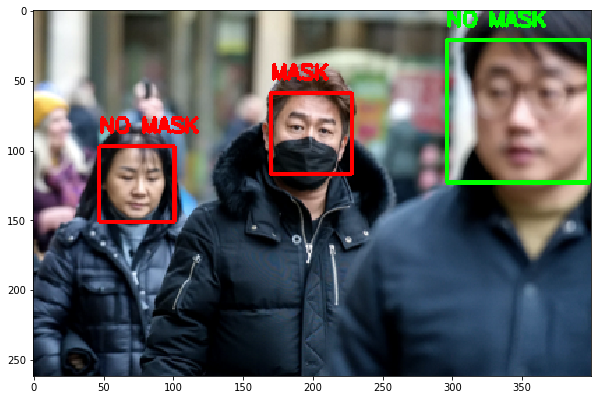
\includegraphics[width=6.26in,height=4.3in]{./media/image10.png}
	\end{Center}
\end{figure}


%%%%%%%%%%%%%%%%%%%% Figure/Image No: 3 Ends here %%%%%%%%%%%%%%%%%%%%


\vspace{\baselineskip}\begin{Center}
Fig 2: Output of mask and social distancing models
\end{Center}
\begin{Center}
 
\end{Center}
\begin{Center}
 
\end{Center}
\begin{Center}
 
\end{Center}
\begin{justify}
Bird\ Eye\ View transformation technique is used  to generate a top view perspective of an image. The Bird’s eye view model increases the area visibility, increasing the efficiency. The Detectron 2.0-based bird's eye view model can potentially detect where each person is in real time and return a bounding box that turns red if two people are dangerously near. The proximity distance refers to the minimum distance between two individuals, and the proximity distance threshold is set to 100. The video-stream can be fetched from any CCTV camera installed in malls, shops, and roads.  As shown in Fig 3, the blue rectangle indicates that the social distance is followed, while 1 and 0 are near and are red rectangles stating that they are potentially close to each other, that is the violation of social distancing.
\end{justify}
\vspace{\baselineskip}
\vspace{\baselineskip}


%%%%%%%%%%%%%%%%%%%% Figure/Image No: 4 starts here %%%%%%%%%%%%%%%%%%%%

\begin{figure}[H]
	\begin{Center}
		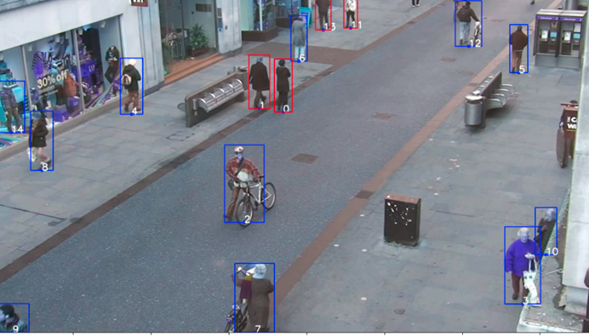
\includegraphics[width=6.14in,height=4.0in]{./media/image7.png}
	\end{Center}
\end{figure}


%%%%%%%%%%%%%%%%%%%% Figure/Image No: 4 Ends here %%%%%%%%%%%%%%%%%%%%

\begin{justify}
 
\end{justify}
\begin{Center}
Fig 3: Bird’s eye view using Detectron 2.0
\end{Center}
\begin{justify}
 
\end{justify}

\vspace{\baselineskip}
\setlength{\parskip}{9.96pt}

\vspace{\baselineskip}
\setlength{\parskip}{12.0pt}
\setlength{\parskip}{9.96pt}
\setlength{\parskip}{12.0pt}
\begin{justify}
{\fontsize{14pt}{16.8pt}\selectfont \textbf{4.2 Active Model Output}}
\end{justify}
\begin{justify}
In the active phase, when the passive models have calculated the most affected user, the mail will only be sent to the person with higher risk. In case the social distance is violated an effective measure is taken. The mail is sent through gmail. Fig 4 shows the output of the mail received. The mail can be edited as per the requirement. The mail sent to the infected person has the link to the chatbot with the consequent CovidDisesaseAsisistant ID CDA-ID. 
\end{justify}
\begin{justify}
{\fontsize{14pt}{16.8pt}\selectfont \textbf{ }}
\end{justify}


%%%%%%%%%%%%%%%%%%%% Figure/Image No: 5 starts here %%%%%%%%%%%%%%%%%%%%

\begin{figure}[H]
	\begin{Center}
		
\includegraphics[width=6.3in,height=2.09in]{./media/image9.png}
	\end{Center}
\end{figure}


%%%%%%%%%%%%%%%%%%%% Figure/Image No: 5 Ends here %%%%%%%%%%%%%%%%%%%%

\begin{Center}
Fig 4: Email received by high-risk
\end{Center}
\begin{justify}
Fig 5 demonstrates a sample chat with a patient, where CDA-ID number $``$123456$"$  has a high risk factor and CDA-ID number $``$234567$"$  is comparatively safe. The chatbot recognises the patient with the respect to their CDA-ID and inquiries for the symptoms that the patient is suffering from and consequently will provide the equivalent remedy. As shown below the bot inquires about the CDA-ID from the patient. As per the CDA-ID the person is recognised. The bot asks for healthy conditions and other symptoms, to match with the COVID-19 symptoms and take the resultant actions. If the symptoms are adverse it suggests that the patient should book an appointment for health checkup and provides the link for the CDA-BookAppointment website. In case the symptoms are mild the chat-bot suggests that $``$you have been home for most of the past 15 days$"$ . Though for additional safety the CDA chatBot suggests to type $``$Yes$"$  for the website link for CDA-BookAppointment.
\end{justify}


%%%%%%%%%%%%%%%%%%%% Figure/Image No: 6 starts here %%%%%%%%%%%%%%%%%%%%


\begin{figure}[H]	\begin{subfigure}		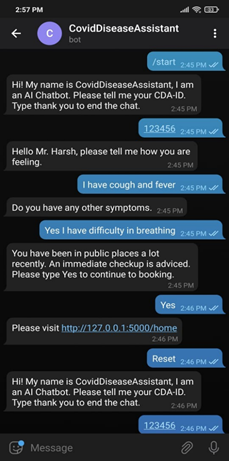
\includegraphics[width=0.45\textwidth,height=6in]{./media/image5.png}
	\end{subfigure}
~	\begin{subfigure}		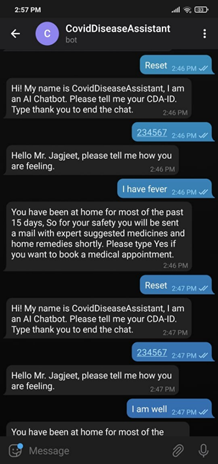
\includegraphics[width=0.45\textwidth,height=6in]{./media/image8.png}
	\end{subfigure}
~
\end{figure}


%%%%%%%%%%%%%%%%%%%% Figure/Image No: 6 Ends here %%%%%%%%%%%%%%%%%%%%


\vspace{\baselineskip}\begin{Center}
Fig 5: CovidDiseaseAssistant ChatBot
\end{Center}

\setlength{\parskip}{9.96pt}
\setlength{\parskip}{12.0pt}
\begin{justify}
The\ Disease Assistant Booking Slot Website Page is shown in Fig 6. The website has a tab for $``$Register$"$  and $``$Login$"$ , and below we can see various days to book the appointment and time slots for individual days. Green slots indicate that they are free , while red slots indicate that they have already been booked. As shown in the figure, Day 2 , 11:00 is booked by CDA-ID $``$12345$"$  and hence no patient can book on that day. If the patient is new he is  required to register else login by using his credentials. Fig 7 is the register page wherein the patient is required to add username and confirm password. The patient can now login with these respective username and password to track their account by clicking the $``$Login$"$  tab henceforth.
\end{justify}


%%%%%%%%%%%%%%%%%%%% Figure/Image No: 7 starts here %%%%%%%%%%%%%%%%%%%%

\begin{figure}[H]
	\begin{Center}
		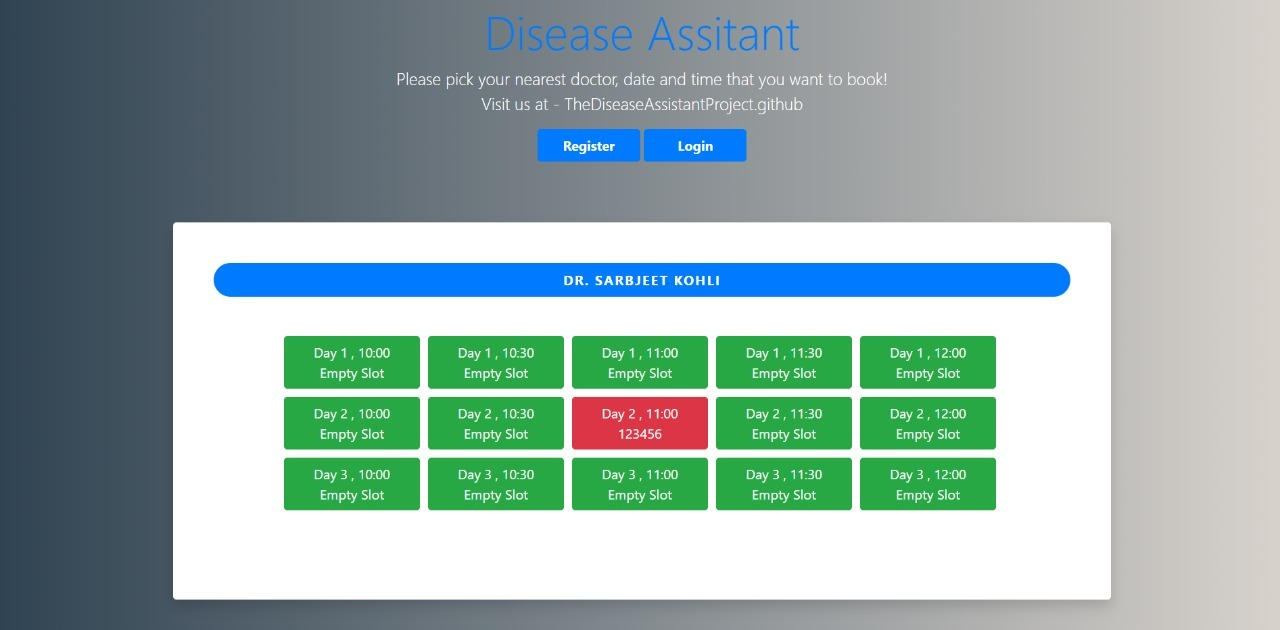
\includegraphics[width=6.52in,height=3.33in]{./media/image2.png}
	\end{Center}
\end{figure}


%%%%%%%%%%%%%%%%%%%% Figure/Image No: 7 Ends here %%%%%%%%%%%%%%%%%%%%


\vspace{\baselineskip}\begin{Center}
Fig 6: Disease Assistant Booking Slot Website Page
\end{Center}

\vspace{\baselineskip}
\setlength{\parskip}{9.96pt}


%%%%%%%%%%%%%%%%%%%% Figure/Image No: 8 starts here %%%%%%%%%%%%%%%%%%%%

\begin{figure}[H]
	\begin{Center}
		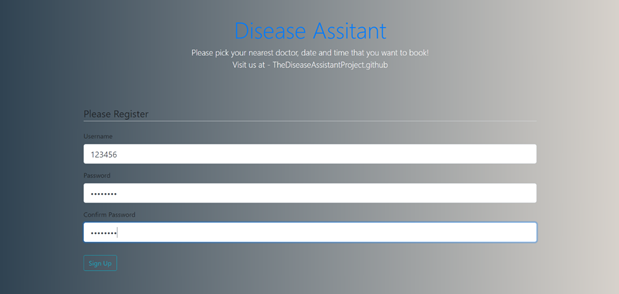
\includegraphics[width=6.49in,height=3.31in]{./media/image13.png}
	\end{Center}
\end{figure}


%%%%%%%%%%%%%%%%%%%% Figure/Image No: 8 Ends here %%%%%%%%%%%%%%%%%%%%

\setlength{\parskip}{12.0pt}

\vspace{\baselineskip}\begin{Center}
Fig 7: Register Page of Disease Assistant Booking Slot Website
\end{Center}

\vspace{\baselineskip}
\setlength{\parskip}{9.96pt}

\vspace{\baselineskip}
\setlength{\parskip}{12.0pt}
\setlength{\parskip}{9.96pt}


%%%%%%%%%%%%%%%%%%%% Figure/Image No: 9 starts here %%%%%%%%%%%%%%%%%%%%

\begin{figure}[H]
	\begin{Center}
		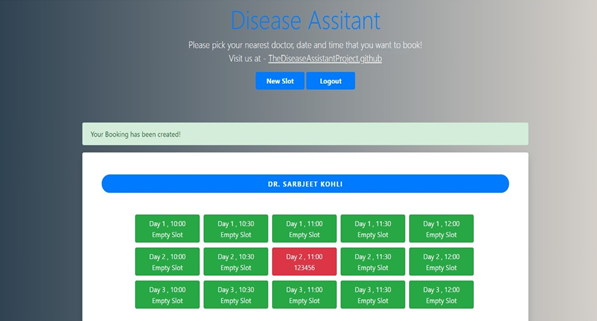
\includegraphics[width=6.22in,height=3.01in]{./media/image12.png}
	\end{Center}
\end{figure}


%%%%%%%%%%%%%%%%%%%% Figure/Image No: 9 Ends here %%%%%%%%%%%%%%%%%%%%

\setlength{\parskip}{12.0pt}
\begin{Center}
Fig 8: After Register page of Disease Assistant Booking Slot Website
\end{Center}
\begin{justify}
Fig\ 8\ shows the output of the after registered page. The green slots indicate that they are empty and can be booked with the desired timings whereas the  red slots indicate that they have been already booked by  CDA-ID ‘123456’ on Day 2, 11:00. A particular account needs to simply click on the desired slot, as shown in Fig 9 and press the Book button. It also shows the desired slot to be booked, that is Day 1, 10:00 to be booked, and confirm by pressing BooK button.
\end{justify}


%%%%%%%%%%%%%%%%%%%% Figure/Image No: 10 starts here %%%%%%%%%%%%%%%%%%%%

\begin{figure}[H]
	\begin{Center}
		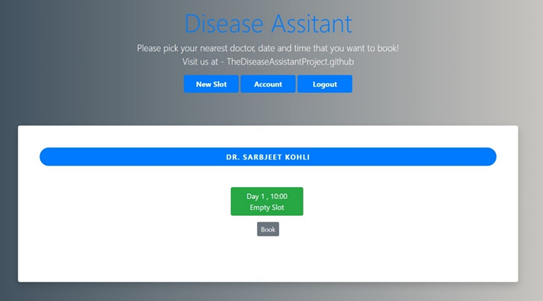
\includegraphics[width=6.14in,height=3.14in]{./media/image11.png}
	\end{Center}
\end{figure}


%%%%%%%%%%%%%%%%%%%% Figure/Image No: 10 Ends here %%%%%%%%%%%%%%%%%%%%

\begin{Center}
Fig 9: Booking slot Day 1 Page
\end{Center}
\begin{justify}
When the $``$Book$"$  button is pressed Fig 10 shows the New booking page. The patient needs to add the Name or CDA-ID and click on Done. Fig 11 shows the output after booking the Day 1 10:00 slot is red indicating that it is booked by CDA-ID ‘234567’. Hence the slot was successfully booked.
\end{justify}


%%%%%%%%%%%%%%%%%%%% Figure/Image No: 11 starts here %%%%%%%%%%%%%%%%%%%%

\begin{figure}[H]
	\begin{Center}
		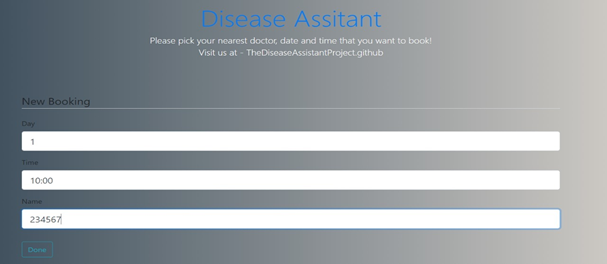
\includegraphics[width=6.3in,height=3.1in]{./media/image6.png}
	\end{Center}
\end{figure}


%%%%%%%%%%%%%%%%%%%% Figure/Image No: 11 Ends here %%%%%%%%%%%%%%%%%%%%
\begin{Center}
Fig 10: New Booking Page
\end{Center}


%%%%%%%%%%%%%%%%%%%% Figure/Image No: 12 starts here %%%%%%%%%%%%%%%%%%%%

\begin{figure}[H]
	\begin{Center}
		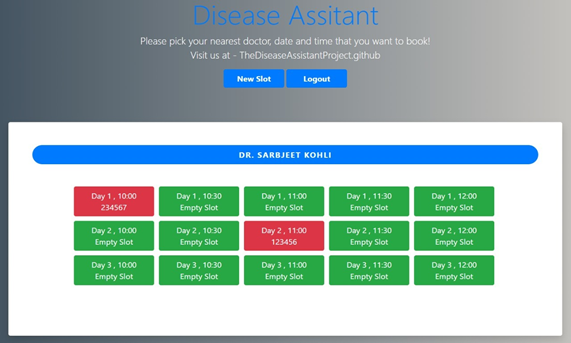
\includegraphics[width=5.99in,height=3.1in]{./media/image3.png}
	\end{Center}
\end{figure}


%%%%%%%%%%%%%%%%%%%% Figure/Image No: 12 Ends here %%%%%%%%%%%%%%%%%%%%

\begin{Center}
 
\end{Center}
\begin{Center}
Fig 11: After Booking Day1 slot by CDA-ID 234567
\end{Center}
\begin{Center}
 {\fontsize{18pt}{21.6pt}\selectfont \textbf{Chapter 5 - Conclusion and Future Scope}}
\end{Center}
\vspace{\baselineskip}
\vspace{\baselineskip}
\setlength{\parskip}{0.0pt}
\begin{justify}
\ The proposed disease assistant model is successful in eliminating social distancing as well as facial detection problems. It successfully recognized objects using the Haar Cascade trained model and gave an accurate proximity measure. The MobileNetV2 and Transfer learning used gives the best results for feature extraction. The accuracy of the system combining both the facial detection and social distancing model comes out to be high. The bird's eye view model is successfully implemented using Detectron 2.0.  It also consists of a passive approach used to calculate the risk factor based on various risk parameters. The Telegram Chat-bot used makes the interfacing extremely user friendly. It also directs the user to an easy appointment booking software.This model will help in preventing infectious diseases, increasing general hygiene as well as prove to be extremely helpful in pandemic scenarios. 
\end{justify}

\vspace{\baselineskip}
\setlength{\parskip}{9.96pt}
\setlength{\parskip}{0.0pt}
\begin{justify}
 Disease Assistant algorithms will be applied parallely to multiple images of the same place and the results will be combined to get the most precise output as well as parallel analysis ensures no disagreement is caused between models. The system uses very less database power, as it clears memory once the object is out of scope. Day to day functions are handled by the processor on a local computation environment (EDGE technology) which helps speed up the system. The system can be controlled and edited using a very interactive UI which is simple to understand by the end user. The feedback of the effectiveness of the solution will update the database, so that our technology adapts to the changes in the pattern of spreading of diseases under different conditions. 
\end{justify}

\vspace{\baselineskip}
\setlength{\parskip}{9.96pt}
\setlength{\parskip}{0.0pt}
\begin{justify}
The system can be used for targeting the common communicable ailments and ensuring general hygiene is maintained in public places where social interaction is at a peak. It can be further modified to successfully target a specific disease very easily and ensure maximum accuracy and quick adaptation since all the major parameters are accounted for in the base system. A disease becomes a pandemic upon negligence and high infectivity. This system can be successfully implemented as safety and an effective preventive system.
\end{justify}

\vspace{\baselineskip}
\setlength{\parskip}{9.96pt}

\vspace{\baselineskip}
\setlength{\parskip}{0.0pt}
\setlength{\parskip}{9.96pt}

\vspace{\baselineskip}
\setlength{\parskip}{0.0pt}
\setlength{\parskip}{9.96pt}
\vspace{\baselineskip}
\vspace{\baselineskip}
\vspace{\baselineskip}
\vspace{\baselineskip}
\vspace{\baselineskip}
\vspace{\baselineskip}
\vspace{\baselineskip}
\vspace{\baselineskip}
\vspace{\baselineskip}
\vspace{\baselineskip}
\vspace{\baselineskip}
\vspace{\baselineskip}
\vspace{\baselineskip}

\begin{Center}
{\fontsize{18pt}{21.6pt}\selectfont \textbf{References}}
\end{Center}
\vspace{\baselineskip}
\begin{justify}
[1] M. S. Ejaz and M. R. Islam, "Masked Face Recognition Using Convolutional Neural Network," 2019 International Conference on Sustainable Technologies for Industry 4.0 (STI), Dhaka, Bangladesh, 2019, pp. 1-6, doi: 10.1109/STI47673.2019.9068044.
\end{justify}
\begin{justify}
 [2] Monitoring COVID-19 social distancing with person detection and tracking via fine-tuned YOLO v3 and Deepsort techniques N. S. Punn, S. K. Sonbhadra, S. Agarwal, Indian Institute of Information Technology Allahabad, Jhalwa, Prayagraj, Uttar Pradesh, India; emails: $ \{ $ pse2017002, rsi2017502,sonali$ \} $ @iiita.ac.in.
\end{justify}
\begin{justify}
 [3] Ghorai, Arnab and Gawde, Sarah and Kalbande, Dhananjay, Digital Solution for Enforcing Social Distancing (May 31, 2020). Proceedings of the International Conference on Innovative Computing $\&$  Communications (ICICC) 2020, Available at SSRN: https://ssrn.com/abstract=3614898 or http://dx.doi.org/10.2139/ssrn.3614898
\end{justify}
\begin{justify}
 [4] Liu Y, Wang Z, Tian Y, Zhou M, Zhou T, Ye K, Zhao Y, Qiu Y, Li J, Ren JA COVID-19 Risk Assessment Decision Support System for General Practitioners: Design and Development Study J Med Internet Res 2020;22(6):e19786.
\end{justify}
\begin{justify}
 [5]Viola, Paul $\&$  Jones, Michael. (2001). Rapid Object Detection using a Boosted Cascade of Simple Features. IEEE Conf Comput Vis Pattern Recognit. 1. I-511. 10.1109/CVPR.2001.990517. 
\end{justify}
\setlength{\parskip}{2.52pt}
\begin{justify}
{\fontsize{10pt}{12.0pt}\selectfont [}6]P. Viola and M. Jones, "Rapid object detection using a boosted cascade of simple features," Proceedings of the 2001 IEEE Computer Society Conference on Computer Vision and Pattern Recognition. CVPR 2001, Kauai, HI, USA, 2001, pp. I-I, doi: 10.1109/CVPR.2001.99051.
\end{justify}
\printbibliography
\end{document}